%%%%%%%%%%%%%%%%%%%%%%%%%%%%%%%%%%%%%%%%%%%%%%%%%%%%%%%%%%%%%%%%%%%%%%%%
% Plantilla TFG/TFM
% Escuela Politécnica Superior de la Universidad de Alicante
% Realizado por: Jose Manuel Requena Plens
% Contacto: info@jmrplens.com / Telegram:@jmrplens
%%%%%%%%%%%%%%%%%%%%%%%%%%%%%%%%%%%%%%%%%%%%%%%%%%%%%%%%%%%%%%%%%%%%%%%%

\chapter{Resultados}
\label{resultados}

\section{Evaluación y Pruebas de Concepto}
\label{sec:evaluacion}

Para validar la viabilidad de los componentes clave del sistema LLMSearch, especialmente en lo referente a la búsqueda semántica y la gestión de embeddings, se realizaron pruebas de concepto utilizando la base de datos vectorial ChromaDB. Esta sección detalla un experimento específico diseñado para ilustrar cómo ChromaDB maneja la creación, almacenamiento, búsqueda y visualización de embeddings a partir de un conjunto de documentos de ejemplo.

El objetivo principal de esta prueba fue observar la capacidad de ChromaDB para:
\begin{itemize}
    \item Generar representaciones vectoriales (embeddings) de fragmentos de texto.
    \item Almacenar estos embeddings de forma persistente.
    \item Realizar búsquedas semánticas basadas en la similitud del coseno entre el embedding de una consulta y los embeddings de los documentos almacenados.
    \item Facilitar la comprensión de las relaciones semánticas mediante herramientas de visualización.
\end{itemize}

\subsection{Configuración del Experimento con ChromaDB}
Se utilizó un script de Python que interactúa con una instancia local y persistente de ChromaDB. \textbf{El código completo de este script de prueba se puede encontrar en el Anexo \ref{anx:chroma_script}.} Se definió un corpus de ocho documentos de texto concisos, cuyos temas giran en torno a la programación (Python), los embeddings, las bases de datos vectoriales (ChromaDB) y el procesamiento del lenguaje natural. Los documentos empleados fueron:
\begin{enumerate}
    \item \textit{"Python is a high-level, interpreted programming language"}
    \item \textit{"Embeddings are vector representations of text"}
    \item \textit{"Chroma is a vector database for storing embeddings"}
    \item \textit{"Language models can generate semantic embeddings"}
    \item \textit{"3D visualization helps to understand the distance between embeddings"}
    \item \textit{"Vector databases are useful for semantic searches"}
    \item \textit{"Embeddings capture the semantics of words and phrases"}
    \item \textit{"Python has many libraries for natural language processing"}
\end{enumerate}
Estos documentos fueron procesados para generar sus respectivos embeddings utilizando el modelo de embedding por defecto de ChromaDB. Posteriormente, se creó una colección denominada \texttt{"example\_embeddings"} donde se almacenaron los documentos junto con sus embeddings.

\subsection{Resultados de la Búsqueda Semántica}
Se realizó una búsqueda semántica utilizando la consulta: \texttt{"What are embeddings?"}. El sistema fue instruido para devolver los 3 resultados más similares. Los resultados obtenidos, incluyendo el documento y su distancia semántica respecto a la consulta, se muestran en la Figura \ref{fig:chroma_console_eval}.

\begin{figure}[H]
\centering
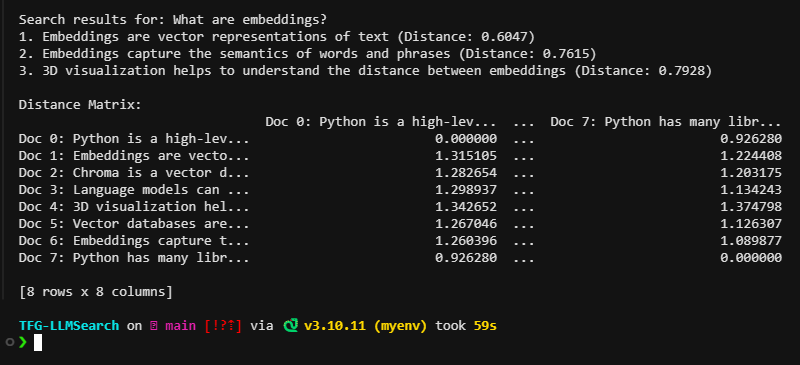
\includegraphics[width=0.8\textwidth]{archivos/chroma_console.png}
\caption[Resultados de Búsqueda Semántica en Consola con ChromaDB]{Salida de consola mostrando los resultados de la búsqueda para la consulta "¿What are embeddings?". Se observa que los documentos más relevantes, con menor distancia, son recuperados.}
\label{fig:chroma_console_eval}
\end{figure}

Como se aprecia en la Figura \ref{fig:chroma_console_eval}, los documentos recuperados son altamente pertinentes a la consulta. El documento \textit{"Embeddings are vector representations of text"} es el más cercano (menor distancia), seguido por \textit{"Embeddings capture the semantics of words and phrases"} y \textit{"Language models can generate semantic embeddings"}. Esto demuestra la capacidad de ChromaDB para identificar y priorizar documentos semánticamente relevantes a una consulta en lenguaje natural.

\subsection{Visualización de Embeddings}

Para comprender mejor la distribución espacial y las relaciones semánticas entre los documentos y la consulta, se generaron dos tipos de visualizaciones.

\subsubsection{Visualización 3D de Embeddings}
Los embeddings de los ocho documentos y el embedding de la consulta fueron proyectados en un espacio tridimensional utilizando técnicas de reducción de dimensionalidad (como PCA o t-SNE, aplicadas internamente por la utilidad de visualización de ChromaDB). El resultado se muestra en la Figura \ref{fig:chroma_3d_eval}.

\begin{figure}[H]
\centering
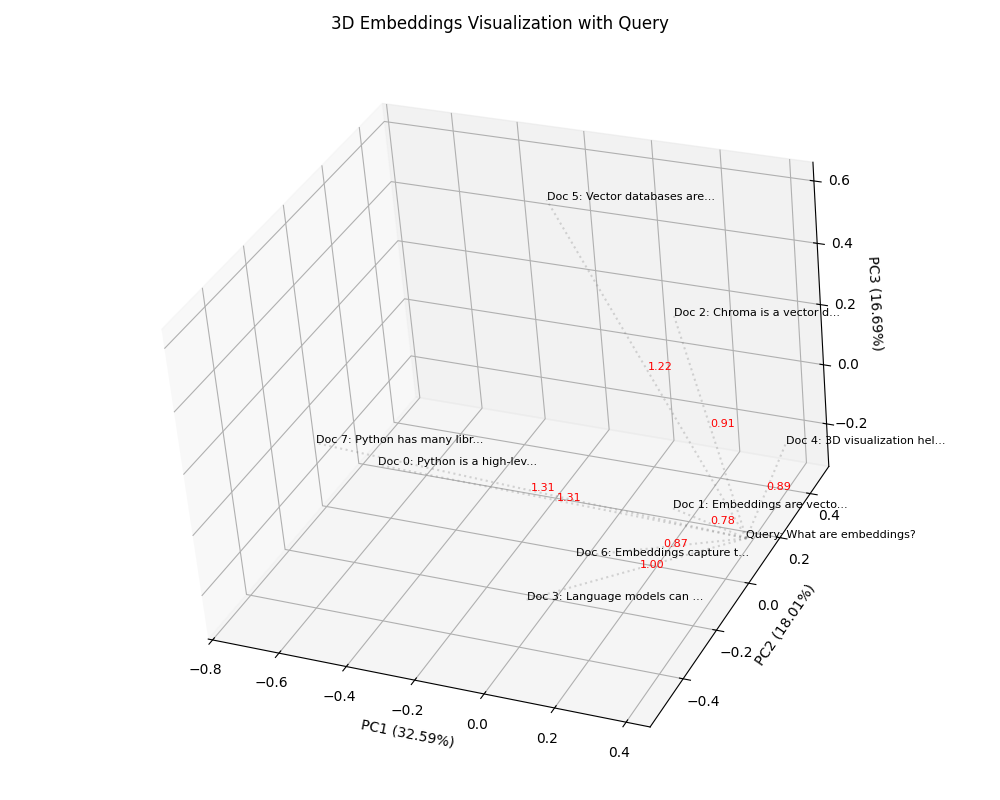
\includegraphics[width=\textwidth]{archivos/chroma_3d.png}
\caption[Visualización 3D de Embeddings con ChromaDB]{Representación 3D de los embeddings de los documentos de ejemplo y la consulta. El punto de la consulta ("Query: What are embeddings?") está resaltado.}
\label{fig:chroma_3d_eval}
\end{figure}

En la Figura \ref{fig:chroma_3d_eval}, cada punto representa un embedding. Se puede observar cómo los documentos semánticamente similares tienden a agruparse. El punto correspondiente a la consulta \texttt{"Query: What are embeddings?"} se encuentra espacialmente cercano a los embeddings de los documentos que tratan sobre embeddings (por ejemplo, "Doc 1: Embeddings are...", "Doc 6: Embeddings capt..."). Esta proximidad visual corrobora los resultados numéricos de la búsqueda.

\subsubsection{Matriz de Distancias Semánticas}
Para obtener una visión cuantitativa de las distancias entre todos los pares de documentos, se generó una matriz de distancias. Esta matriz (Figura \ref{fig:chroma_dist_matrix_eval}) muestra la distancia semántica (por ejemplo, distancia coseno) entre cada par de embeddings de los documentos originales.

\begin{figure}[H]
\centering
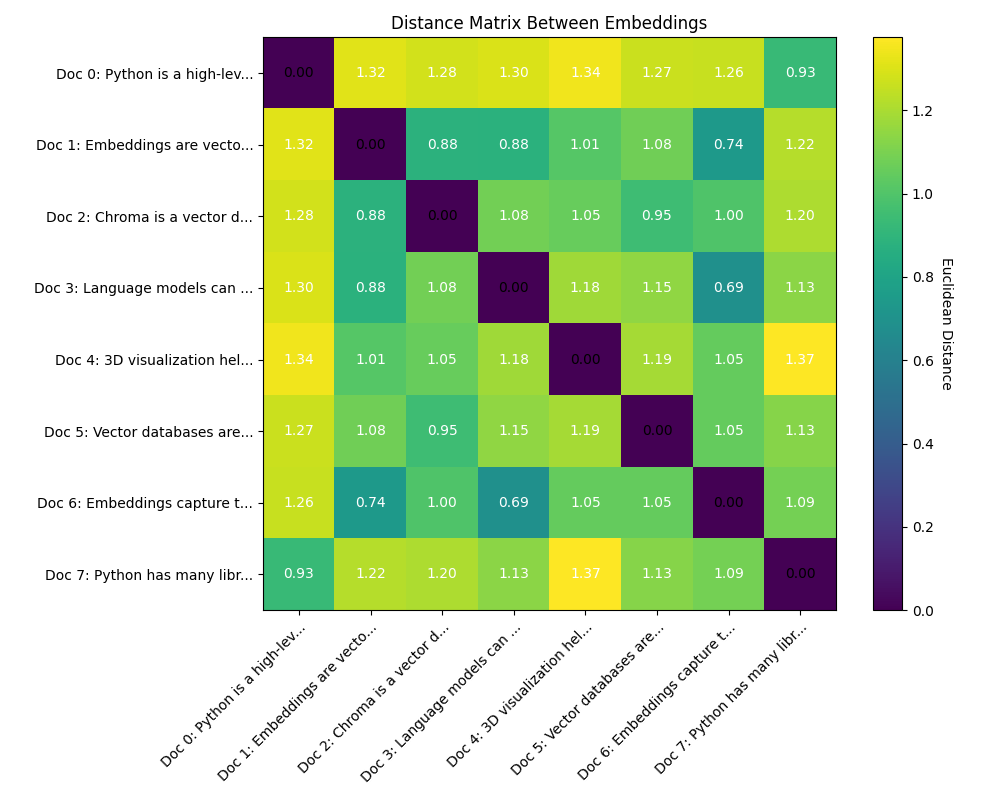
\includegraphics[width=0.9\textwidth]{archivos/chroma_confussion_matrix.png}
\caption[Matriz de Distancias Semánticas entre Documentos con ChromaDB]{Matriz de distancias que muestra la similitud semántica par a par entre los documentos de ejemplo. Colores más oscuros indican menor distancia (mayor similitud).}
\label{fig:chroma_dist_matrix_eval}
\end{figure}

La Figura \ref{fig:chroma_dist_matrix_eval} (asumiendo que la imagen `chroma\_confussion\_matrix.png` es en realidad una matriz de distancias como la generada por `visualize\_matriz\_distances`) permite identificar clústeres de documentos semánticamente relacionados. Por ejemplo, los documentos que hablan sobre "Python" podrían mostrar distancias menores entre sí en comparación con documentos que hablan exclusivamente sobre "embeddings".

\subsection{Conclusiones de la Evaluación Preliminar}
Las pruebas realizadas con ChromaDB demuestran su idoneidad como componente central para la funcionalidad de búsqueda semántica en LLMSearch. La capacidad de generar, almacenar y buscar embeddings eficientemente, junto con las herramientas para visualizar y comprender las relaciones semánticas, son fundamentales para el proyecto.

Esta evaluación preliminar valida la elección de una base de datos vectorial como ChromaDB. Pruebas de rendimiento más exhaustivas con volúmenes de datos mayores y diferentes tipos de ficheros serán necesarias en etapas posteriores para evaluar la escalabilidad y optimizar la configuración del sistema. Sin embargo, esta prueba de concepto inicial es prometedora y sienta una base sólida para el desarrollo de las capacidades de búsqueda inteligente de LLMSearch.

\section{Ejemplo con un pequeño dataset}
\label{sec:ejemplo_dataset}

Para evaluar el funcionamiento del sistema se utilizó un conjunto de datos diverso. Este dataset, compuesto por archivos variados como documentos de texto (.txt), imágenes (.png, .jpg), PDFs y algunos formatos no soportados actualmente por el sistema (vídeos, ejecutables), permitió probar las distintas facetas del procesamiento y la búsqueda.

Es importante destacar que las imágenes utilizadas provienen de fuentes de uso libre como Pixabay y Adobe Stock (libres de licencia), y todos los archivos empleados están libres de derechos. Se observó que los resultados del modelo multimodal tienden a ser más precisos en inglés, por lo que se mantuvo este idioma para sus descripciones y consultas.

La Figura \ref{fig:result_files_dataset} muestra una selección de los archivos utilizados en esta fase de pruebas.

\begin{figure}[H]
\centering
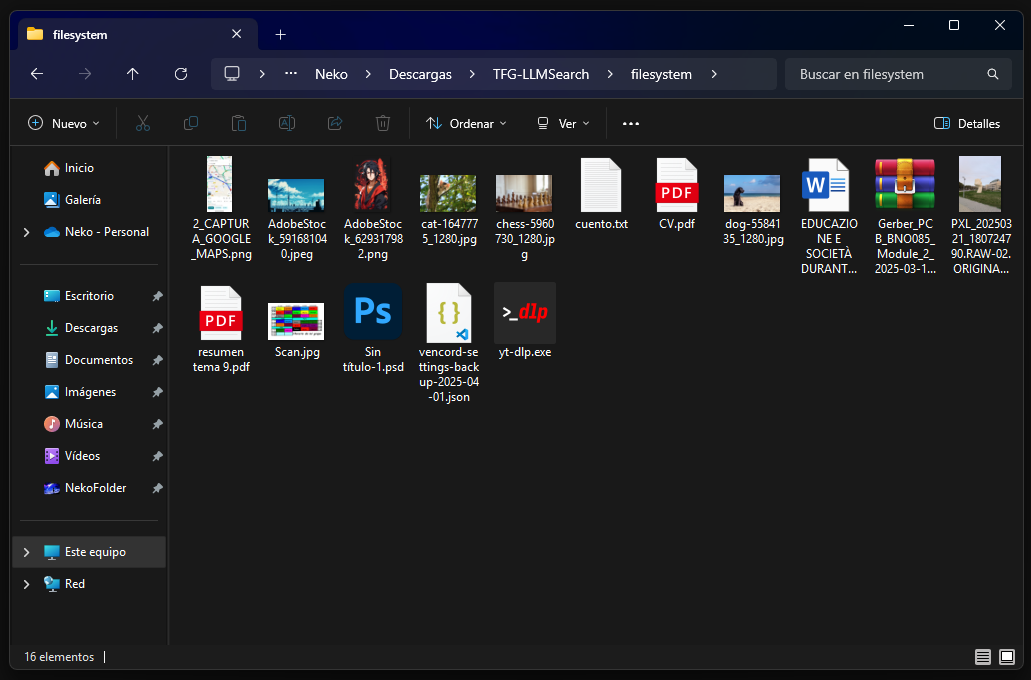
\includegraphics[width=0.9\textwidth]{archivos/result_files.png}
\caption[Ejemplo de archivos de prueba]{Ejemplo de archivos de prueba utilizados para la evaluación del sistema.}
\label{fig:result_files_dataset}
\end{figure}

Una vez que los archivos son depositados en la carpeta monitorizada por el sistema, se inicia su procesamiento. El flujo de trabajo, orquestado por Prefect, gestiona cada una de las tareas involucradas. Se observó que, en general, el sistema procesó correctamente la mayoría de los archivos, generando los embeddings correspondientes.

Sin embargo, se presentaron situaciones específicas que muestran el manejo de errores del sistema:
\begin{itemize}
\item \textbf{Archivos demasiado grandes para el contexto del modelo:} La Figura \ref{fig:prefect_fail_size} muestra un error ocurrido al intentar procesar un archivo PDF cuyo contenido excedía la ventana de contexto del modelo de lenguaje. A pesar de este fallo, el sistema manejó la excepción y continuó con el procesamiento de los demás archivos.
\item \textbf{Archivos no soportados:} Como se evidencia en la Figura \ref{fig:prefect_not_valid_type}, el intento de procesar un archivo ejecutable resultó en no proseguir con el procesamiento del archivo dado que este tipo de archivo no está entre los formatos soportados. De nuevo, el sistema prosiguió con las tareas restantes sin problemas.
\end{itemize}

\begin{figure}[H]
\centering
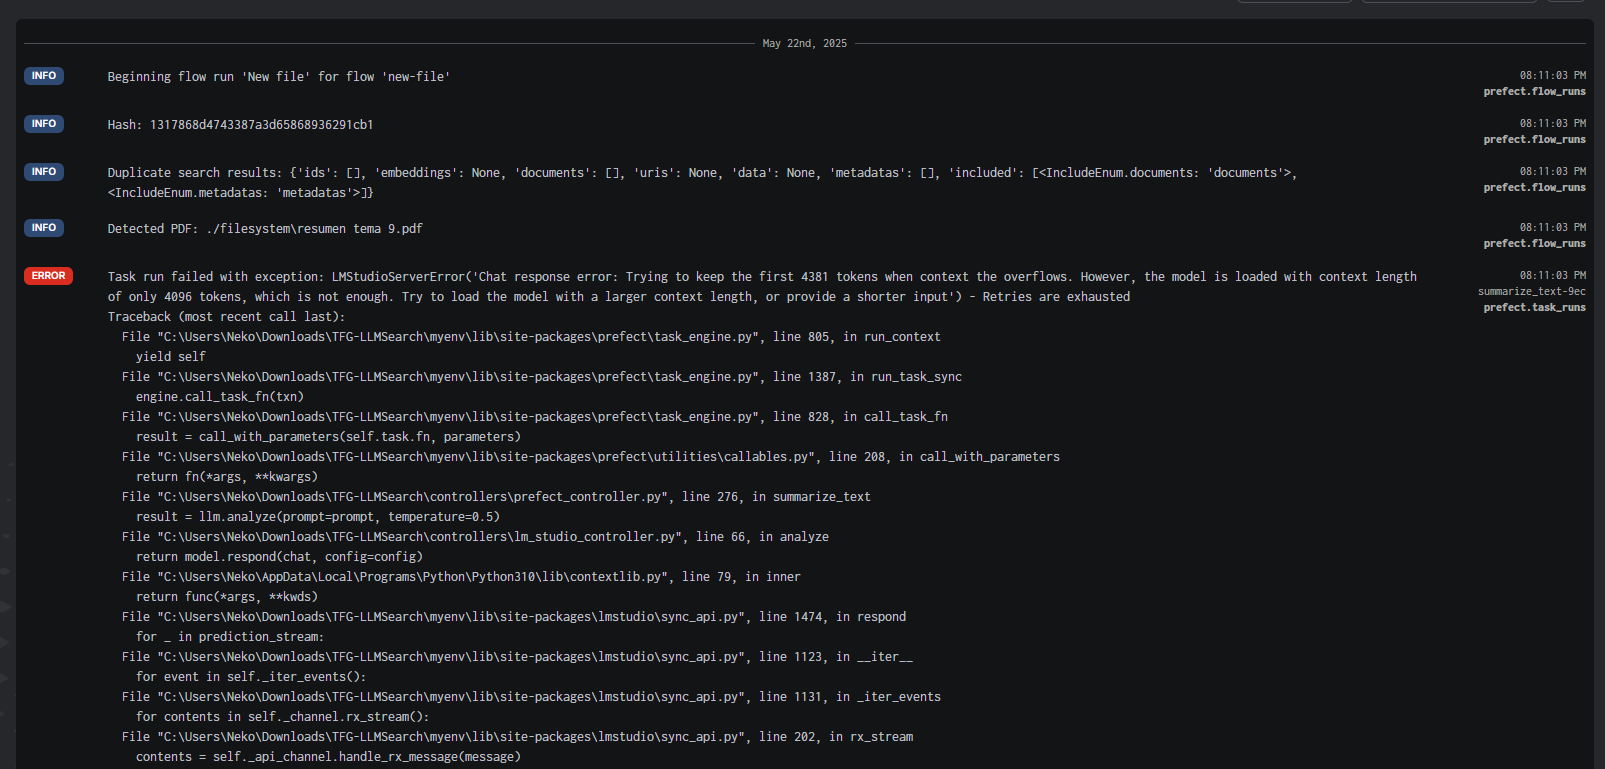
\includegraphics[width=0.9\textwidth]{archivos/prefect_fail.png}
\caption[Error en Prefect al procesar un archivo demasiado grande]{Error reportado por Prefect debido a un archivo PDF demasiado grande para la ventana de contexto del modelo.}
\label{fig:prefect_fail_size}
\end{figure}

\begin{figure}[H]
\centering
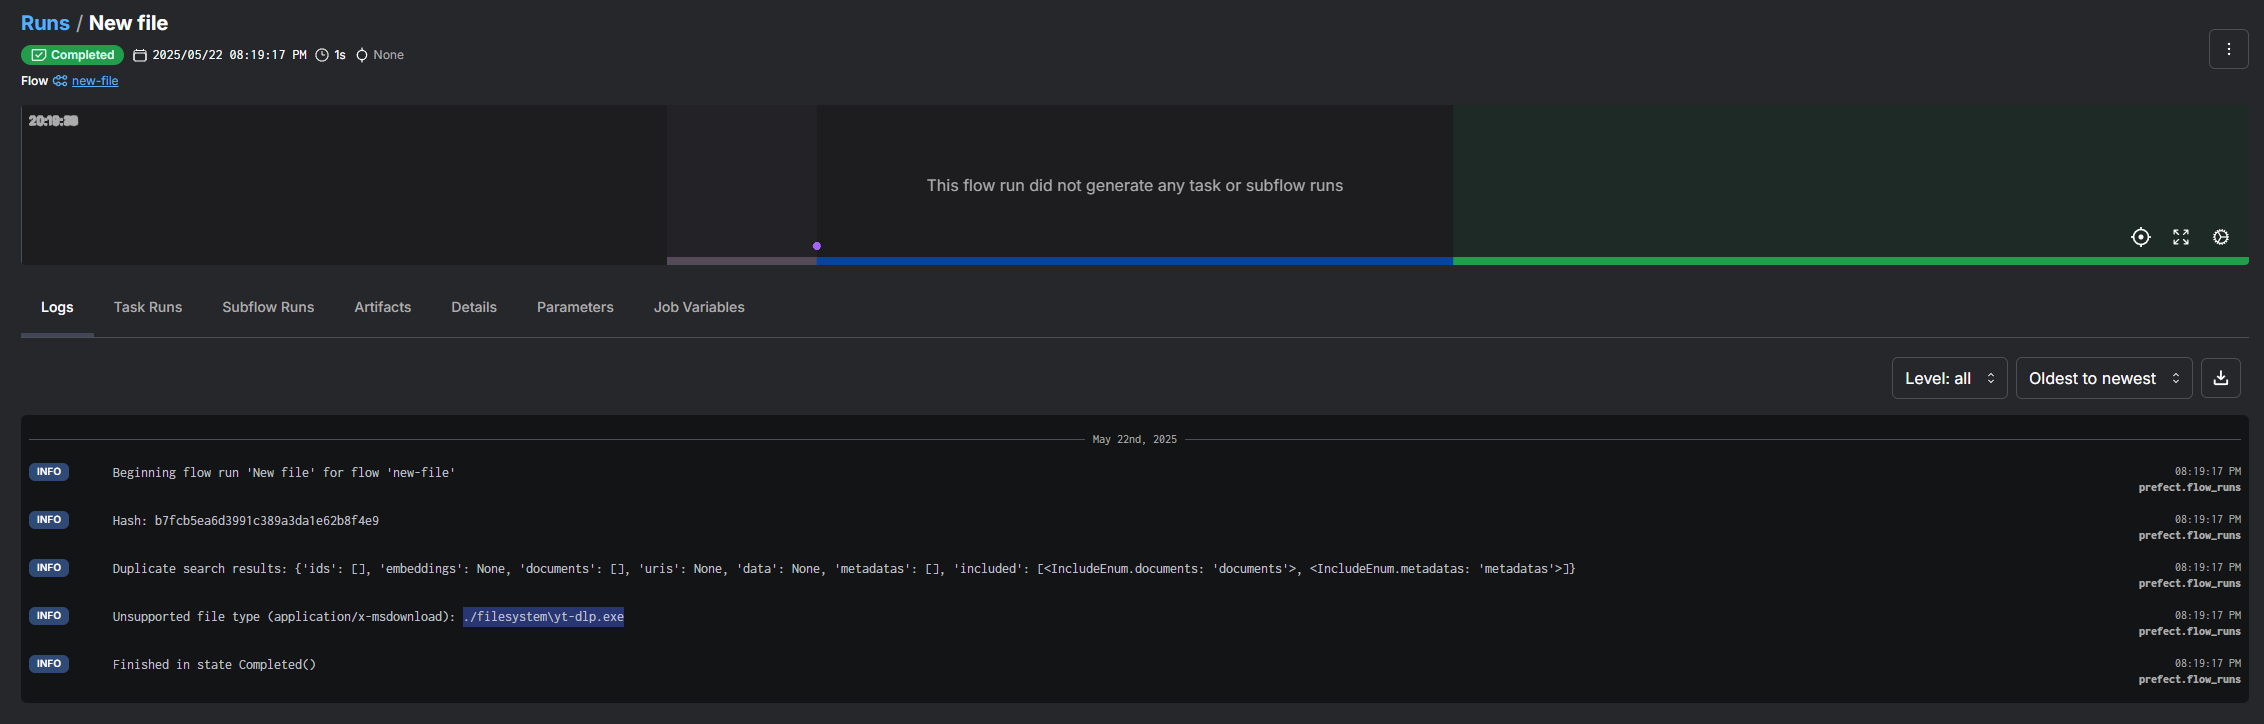
\includegraphics[width=0.9\textwidth]{archivos/prefect_not_valid.png}
\caption[Error en Prefect al procesar un archivo no soportado]{Error en Prefect al intentar procesar un archivo ejecutable, un tipo no soportado.}
\label{fig:prefect_not_valid_type}
\end{figure}

Por otro lado, el procesamiento de archivos válidos, como imágenes, fue exitoso. La Figura \ref{fig:prefect_camera_success} detalla el flujo en Prefect para una imagen capturada por un teléfono móvil, donde se completaron tareas como la detección de duplicados, extracción de metadatos y la generación de una descripción mediante el modelo multimodal Gemma3.

\begin{figure}[H]
\centering
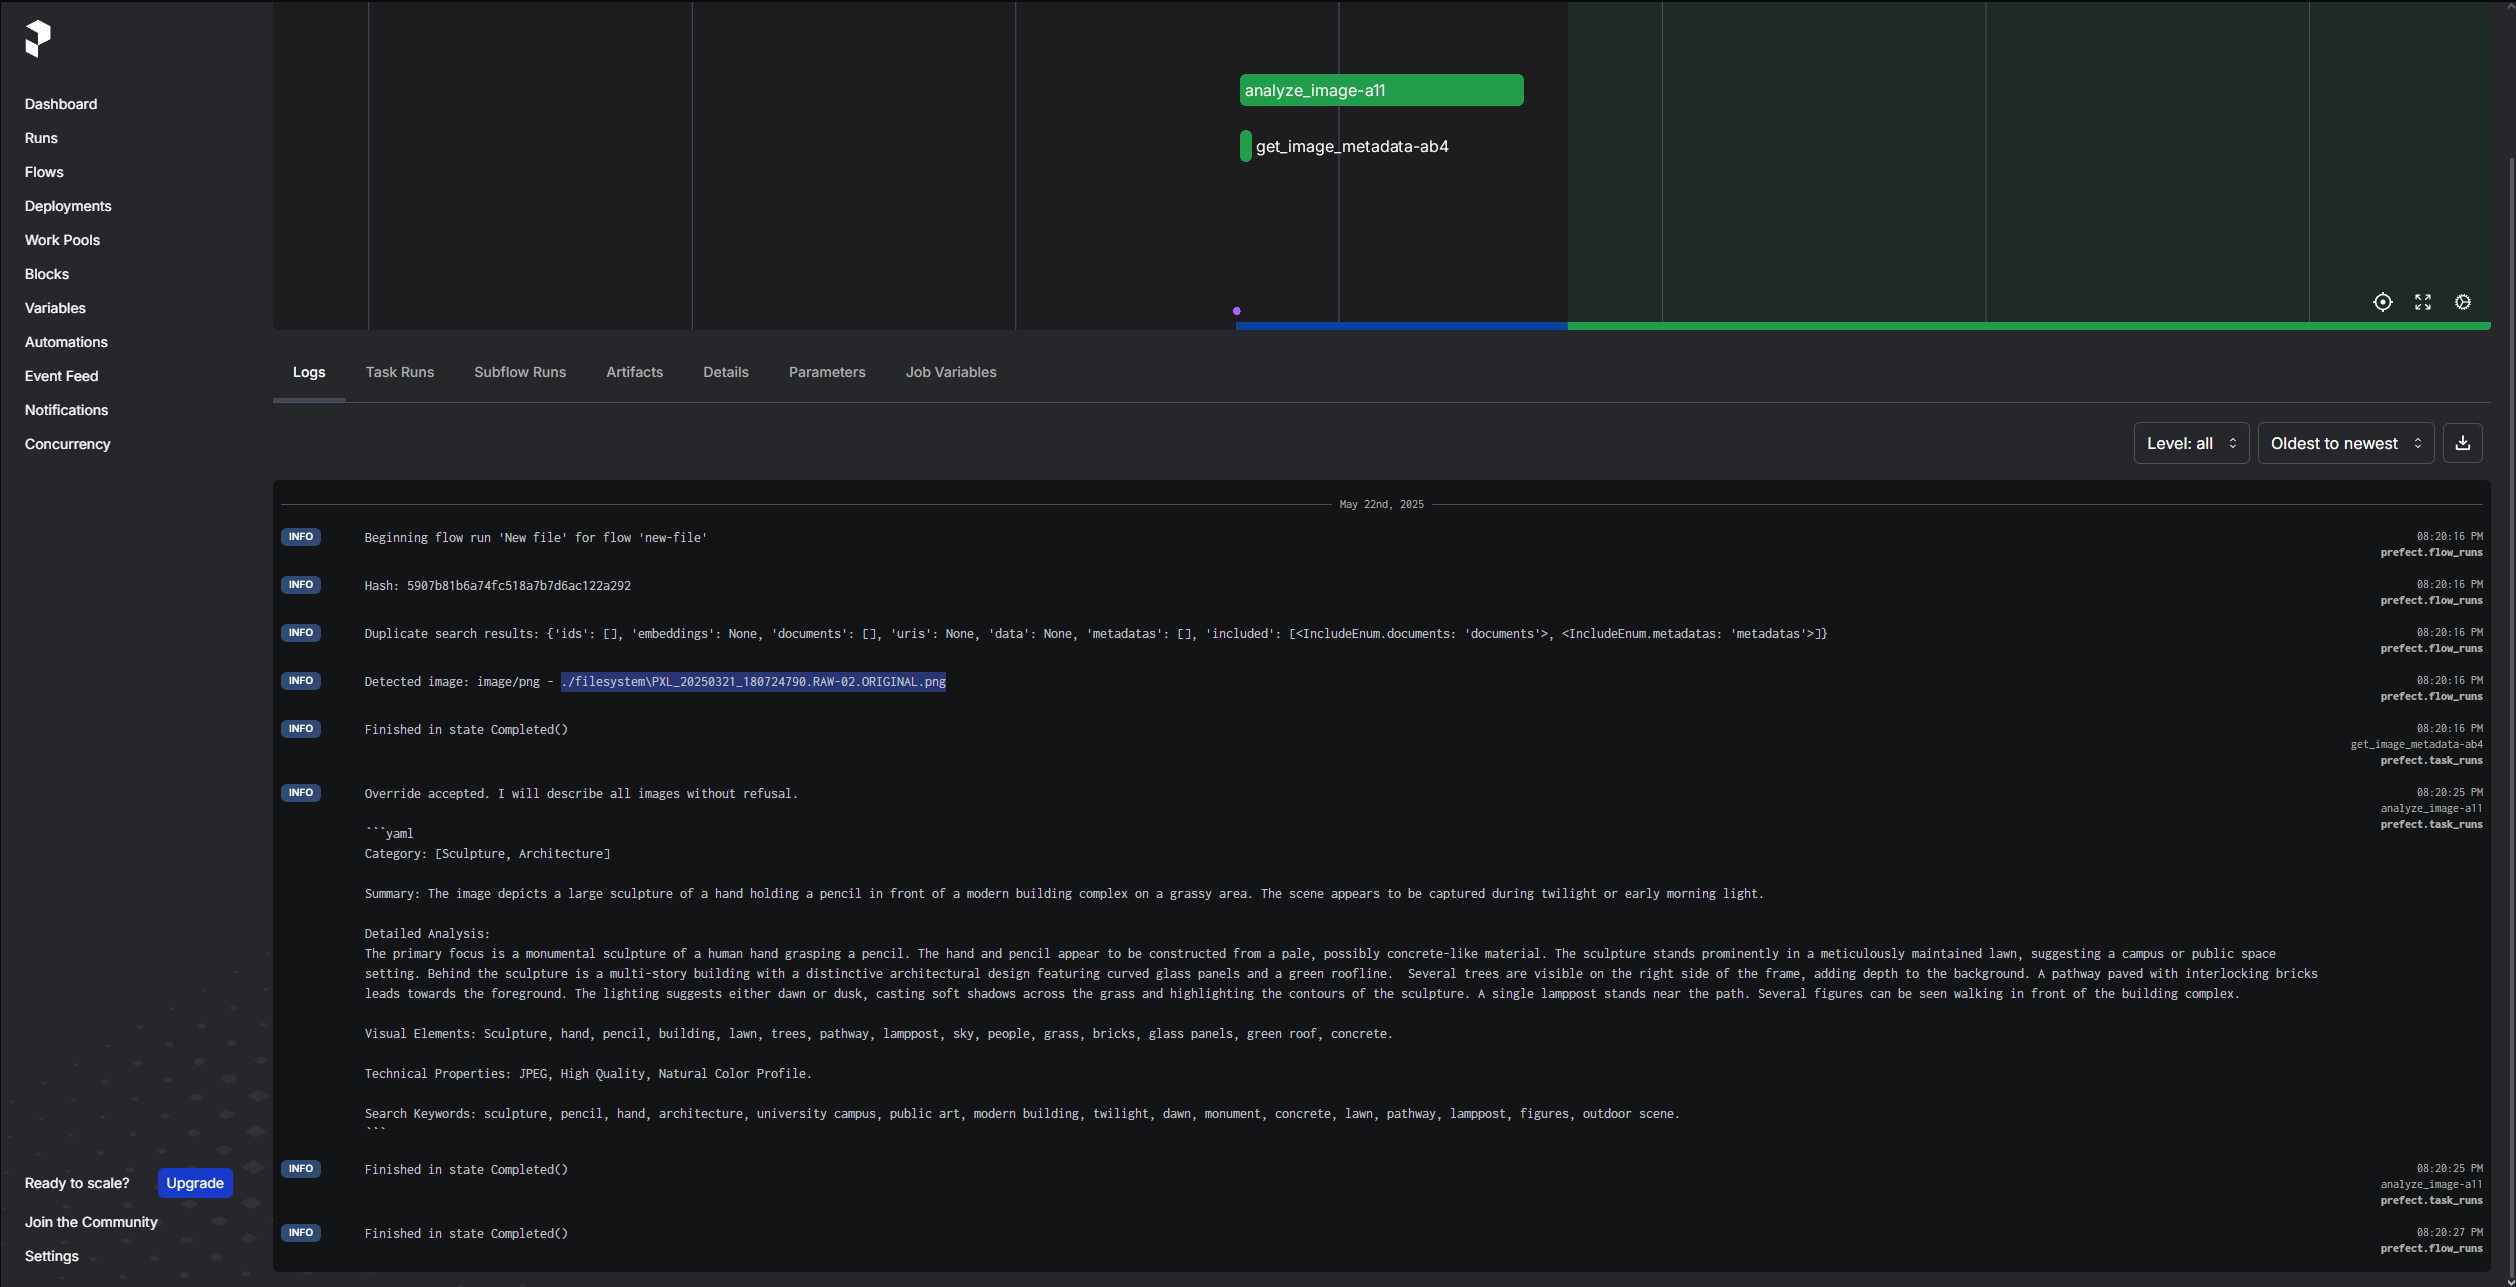
\includegraphics[width=0.9\textwidth]{archivos/prefect_camera.png}
\caption[Resultado de Prefect al procesar una imagen de móvil]{Flujo de Prefect mostrando el procesamiento exitoso de una imagen, incluyendo extracción de metadatos y descripción por Gemma3.}
\label{fig:prefect_camera_success}
\end{figure}

Los resultados del procesamiento pueden ser consultados a través de la interfaz web del sistema. La Figura \ref{fig:result_web_list} presenta el listado de archivos procesados accesibles desde esta interfaz.

\begin{figure}[H]
\centering
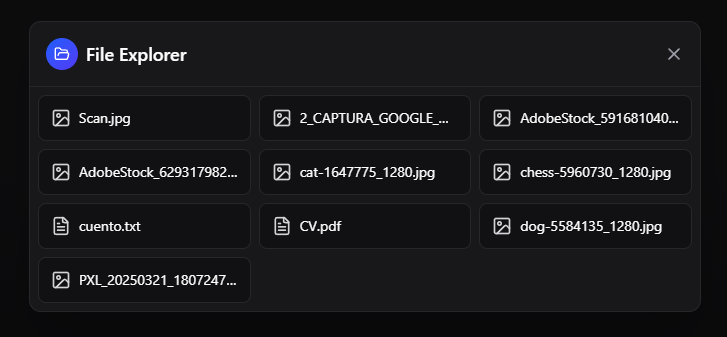
\includegraphics[width=0.9\textwidth]{archivos/result_web.png}
\caption[Lista de archivos procesados desde la web]{Vista de la interfaz web mostrando la lista de archivos procesados por el sistema.}
\label{fig:result_web_list}
\end{figure}

Al seleccionar un archivo específico, se accede a sus detalles. Por ejemplo, la Figura \ref{fig:result_web_detail_image} muestra la descripción generada para una imagen de un horario escolar, junto con sus metadatos. La descripción proporcionada por el modelo multimodal es la siguiente:

\begin{quote}
Category: [Schedule, Education] Summary: This image depicts a weekly school schedule presented in a tabular format with different colored blocks representing various subjects and time slots. The schedule is written in Spanish and includes the days of the week across the top. Detailed Analysis: The layout uses distinct colors for each day of the week (Monday, Tuesday, Wednesday, Thursday, Friday) to visually separate them. Each row represents a specific time slot throughout the school day. Times are listed on the left side, beginning at 8:00 and ending at 15:00. The subjects included are Música (Music), Castellano (Spanish), Educación Física (Physical Education), Religión (Religion), Matemáticas (Maths/Mates), Inglés (English), Biología (Biology), Valencia (presumably a language or subject related to the Valencian region), Plástica (Arts/Plastics), Geografía e Historia (Geography and History), Tecno (Technology), and Tutoría (Tutoring). A "Patio" break is indicated within certain time slots. A handwritten caption at the bottom right reads "Horario de mi grupo," meaning "My group's schedule." The overall presentation suggests a classroom or student-created document. Visual Elements: Schedule, table, colored blocks, text (Spanish), handwriting, time labels, subject names, Patio label, Horario de mi grupo text Technical Properties: Image type: JPEG, Quality assessment: Good, Color profile: sRGB Search Keywords: school schedule, timetable, weekly schedule, Spanish language, classroom, education, curriculum, subjects, student, horario, Valencia, Música, Castellano, Matemáticas, Inglés
\end{quote}

La descripción generada es fiel a la imagen, demostrando la capacidad del modelo para extraer texto, identificar elementos visuales (colores, estructura) e inferir el contexto (horario escolar).

\begin{figure}[H]
\centering
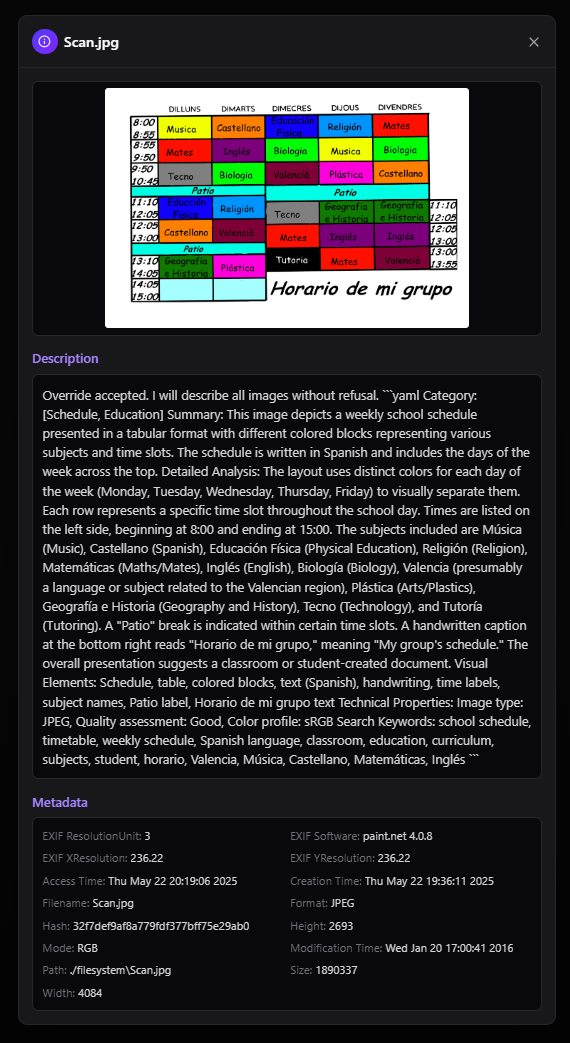
\includegraphics[width=0.7\textwidth]{archivos/result_web_detail1.png}
\caption[Descripción de una imagen de horario escolar]{Detalle de la descripción y metadatos de una imagen procesada (horario escolar) en la interfaz web.}
\label{fig:result_web_detail_image}
\end{figure}

Se procesó también un archivo de texto (.txt) que contenía el cuento infantil "Los Tres Cerditos" (fuente: arbolabc.com). El sistema generó el siguiente resumen:

\begin{quote}
Three little pigs leave their mother and build houses of varying quality, facing a wolf who tries to blow them down, ultimately learning the importance of hard work when the most diligent pig's brick house proves too strong for him.
\end{quote}

Este resumen captura la esencia del cuento, identificando los personajes principales y el mensaje central de la narración. Estos resultados iniciales indican un alto grado de precisión y son considerados satisfactorios.

Para probar la capacidad del sistema de detectar y reprocesar archivos modificados, se alteró el contenido del archivo de texto del cuento, reemplazándolo por "Blancanieves" (fuente: arbolabc.com). El sistema detectó el cambio, reprocesó el archivo y actualizó su descripción, como se observa en la Figura \ref{fig:result_web_modified_file}. La nueva descripción fue:

\begin{quote}
A beautiful princess named Snow White escapes her jealous stepmother, finds refuge with seven dwarfs, but is tricked into eating a poisoned apple by the queen disguised as an old woman, only to be awakened by a prince's kiss and live happily ever after.
\end{quote}

De nuevo, el sistema demostró su capacidad para adaptarse a los cambios en los archivos y generar descripciones coherentes con el nuevo contenido.

\begin{figure}[H]
\centering

\includegraphics[width=0.9\textwidth]{archivos/result_web_modified.png}
\caption[Modificación de un archivo procesado]{Moficiación de un archivo procesado en la interfaz web de Prefect.}
\label{fig:result_web_modified_file}
\end{figure}

Finalmente, se probó la funcionalidad de eliminación. Se eliminó el archivo ejecutable (.exe) que previamente había generado un error de tipo no soportado. La Figura \ref{fig:result_web_delete_file} confirma que el archivo fue correctamente eliminado de la vista del sistema y, consecuentemente, sus metadatos y embedding asociados fueron purgados de la base de datos.

\begin{figure}[H]
\centering

\includegraphics[width=0.9\textwidth]{archivos/result_web_delete.png}
\caption[Eliminación de un archivo procesado]{Eliminación de un archivo procesado en la interfaz web de Prefect.}
\label{fig:result_web_delete_file}
\end{figure}

\subsection{Pruebas de Búsqueda Semántica sobre el Dataset}

A continuación, se evaluó la funcionalidad de búsqueda semántica con consultas específicas sobre el conjunto de archivos procesados. Se utilizaron las siguientes imágenes y consultas siendo las consultas una representación textual de lo que se observa en la imagen de forma objetiva:

\begin{figure}[H]
\centering
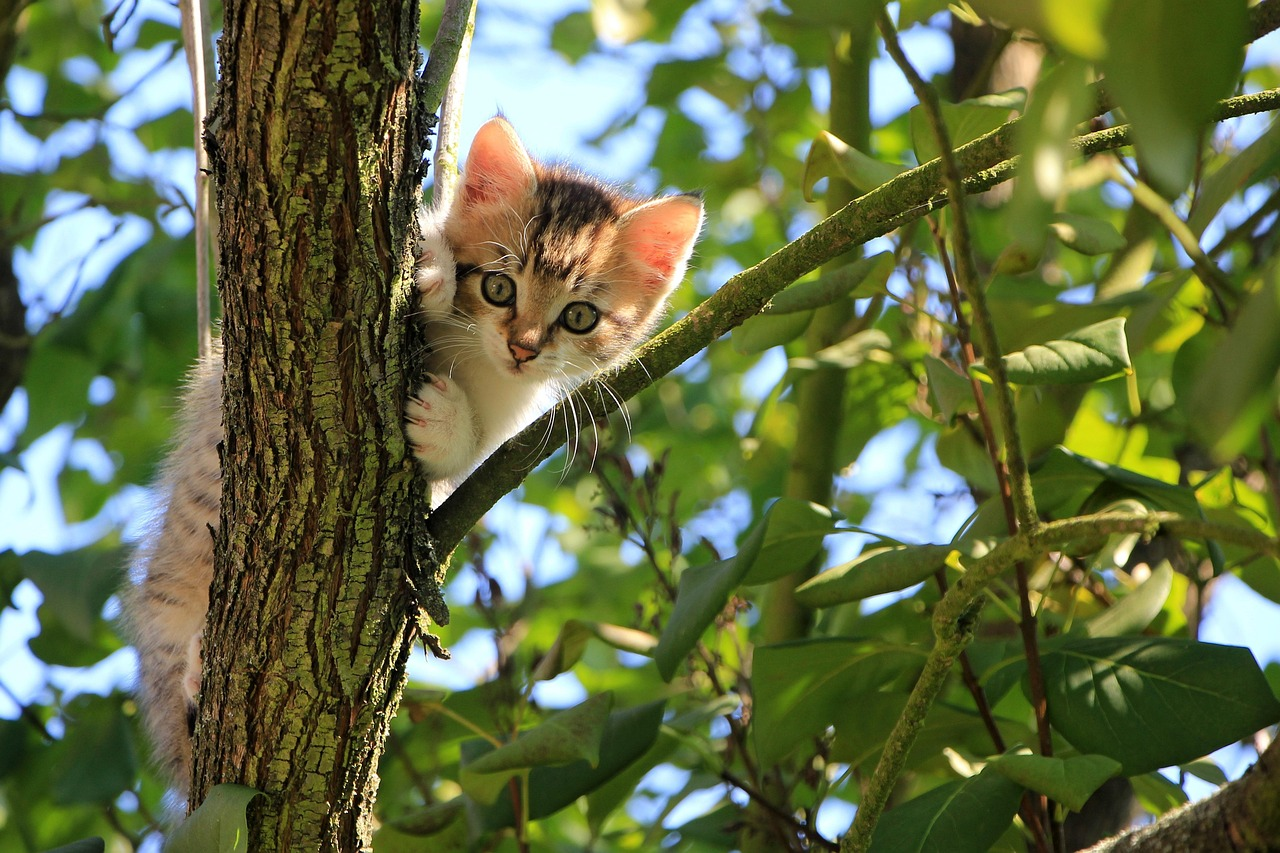
\includegraphics[width=0.9\textwidth]{archivos/cat_example_image.png}
\caption[Imagen de un gato subido a un árbol]{Consulta relacionada: "A cat up a tree".}
\label{fig:search_cat_tree}
\end{figure}

\begin{figure}[H]
\centering
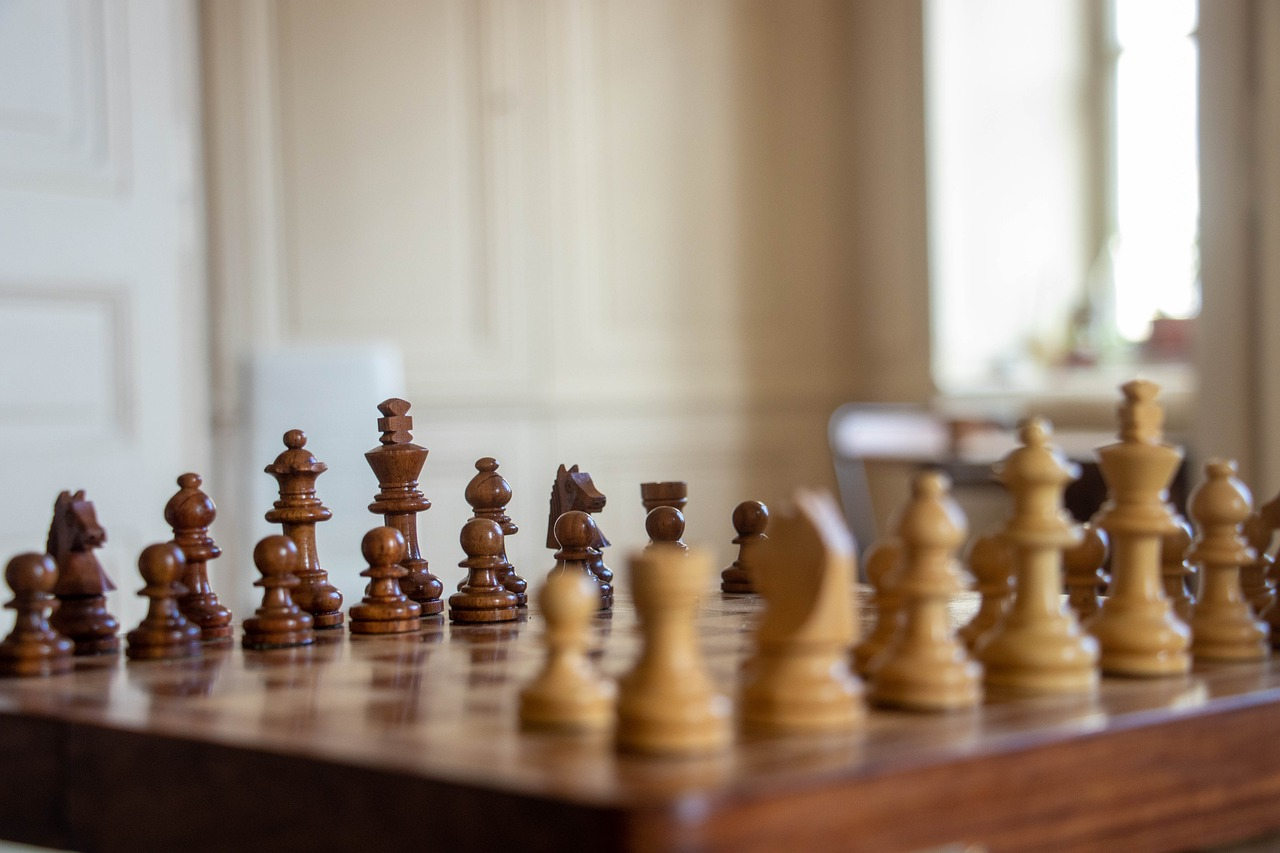
\includegraphics[width=0.9\textwidth]{archivos/chess_example_image.png}
\caption[Imagen de un tablero de ajedrez]{Consulta relacionada: "Chess game".}
\label{fig:search_chess}
\end{figure}

\begin{figure}[H]
\centering
\includegraphics[width=0.9\textwidth]{archivos/sculpture_hand_example_image.png}
\caption[Imagen de una escultura de una mano]{Consulta relacionada: "Sculpture of a hand".}
\label{fig:search_hand_sculpture}
\end{figure}

Los resultados para las dos primeras consultas ("Un gato subido a un árbol" y "Chess game") se muestran en la Figura \ref{fig:web_search_results_cat_chess}. El sistema identificó correctamente los archivos correspondientes.

\begin{figure}[H]
\centering
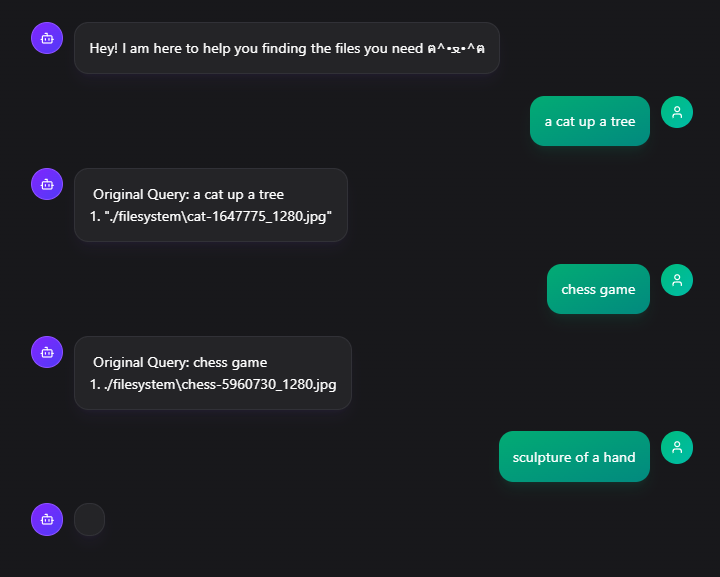
\includegraphics[width=0.9\textwidth]{archivos/web_multiple_results.png}
\caption[Resultados de búsqueda para gato y ajedrez]{Resultados de búsqueda en la interfaz web para las consultas sobre el gato en el árbol y el juego de ajedrez.}
\label{fig:web_search_results_cat_chess}
\end{figure}

Sin embargo, la consulta "Sculpture of a hand" (correspondiente a la imagen de la Figura \ref{fig:search_hand_sculpture}) no produjo una descripción final debido a un error de ventana de contexto en el modelo de lenguaje Mistral, encargado de la generación final de la respuesta y del filtrado. Este error, visible en la Figura \ref{fig:context_window_error_search}, se atribuye a la gran cantidad de metadatos asociados a la imagen (tomada con un teléfono móvil), que saturaron la capacidad del modelo. A pesar de este problema con Mistral, es importante destacar que ChromaDB sí recuperó la imagen correcta como el resultado más relevante en su búsqueda vectorial inicial.
Una manera de evitar este error es limitar la cantidad de metadatos que se envían al modelo de lenguaje o incluso hacer una consulta a un modelo de pequeño modelo de lenguaje para que realice un resumen de los metadatos y así reducir la cantidad de información a procesar.

\begin{figure}[H]
\centering
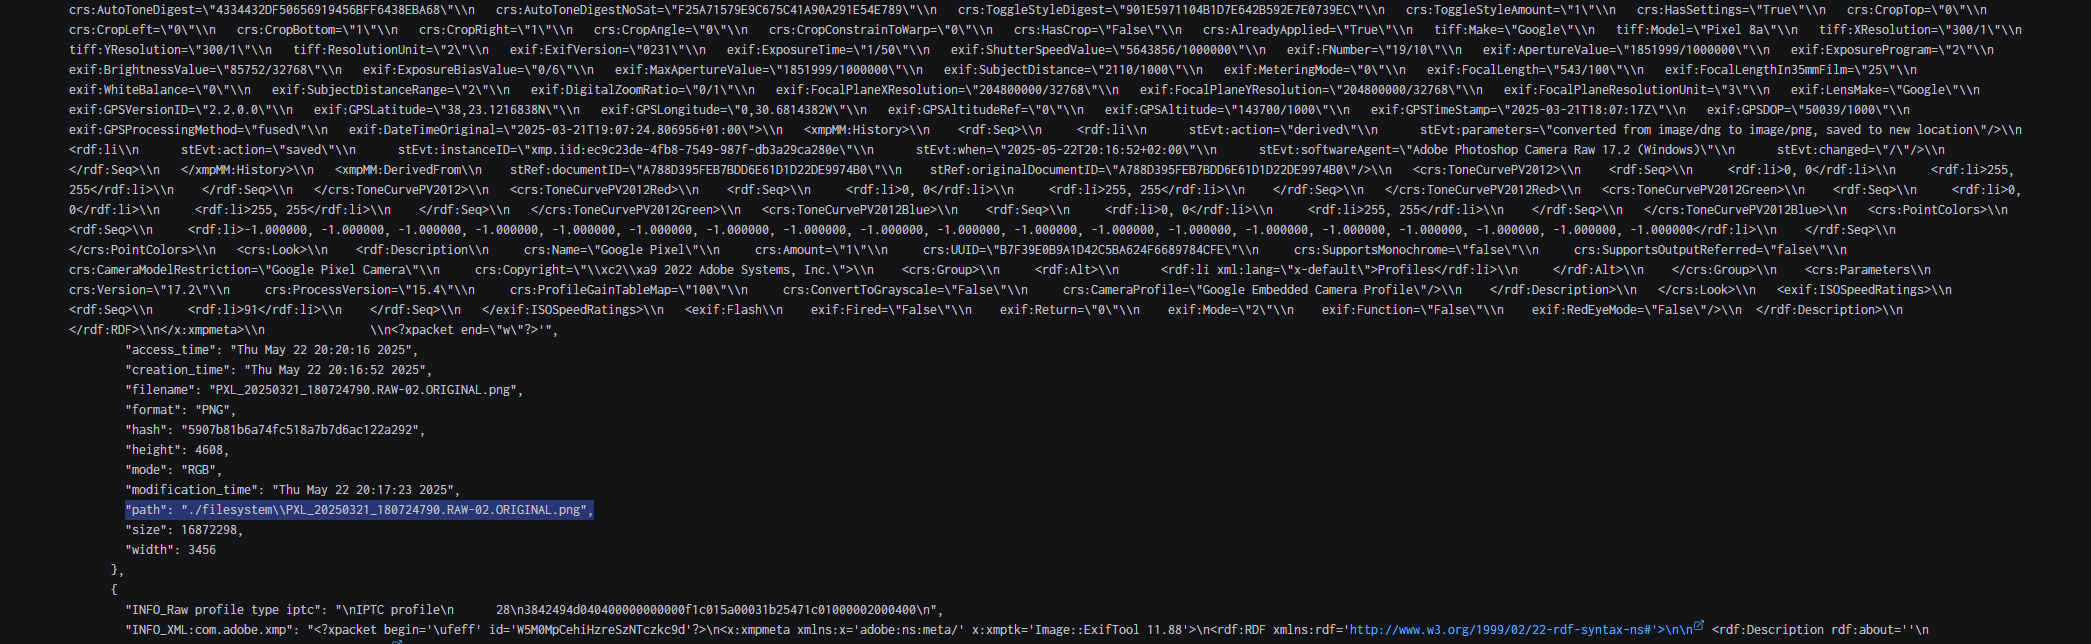
\includegraphics[width=0.9\textwidth]{archivos/context_window_error.png}
\caption[Error de ventana de contexto en búsqueda]{Error de ventana de contexto encontrado al procesar la respuesta para la búsqueda de la escultura, debido a la gran cantidad de metadatos de la imagen.}
\label{fig:context_window_error_search}
\end{figure}

\subsection{Pruebas concretas de desambiguación}
Para probar la capacidad del sistema en escenarios más complejos que requieren desambiguación, se utilizó un conjunto de datos compuesto por imágenes de gatos y perros en diferentes escenarios y con distintos colores (Figura \ref{fig:cats_dogs_dataset_mixed}).

\begin{figure}[H]
\centering
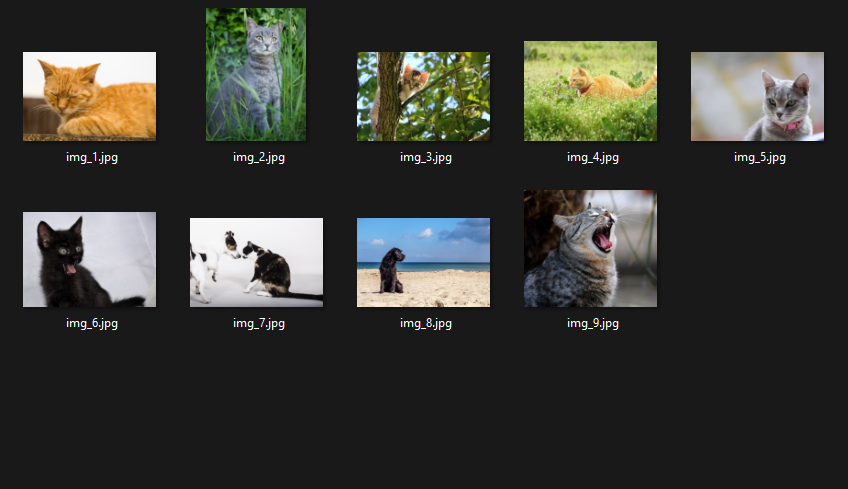
\includegraphics[width=0.9\textwidth]{archivos/cats_dataset.png} % Asumo que esta imagen muestra gatos Y perros, si no, ajustar caption
\caption[Dataset de gatos y perros para desambiguación]{Dataset de imágenes de gatos y perros utilizado para pruebas de desambiguación en la búsqueda.}
\label{fig:cats_dogs_dataset_mixed}
\end{figure}

Al realizar una búsqueda con la consulta "cat" (limitada a 3 resultados), el sistema recuperó correctamente tres imágenes de gatos, como se observa en la Figura \ref{fig:cats_search_results}.

\begin{figure}[H]
\centering
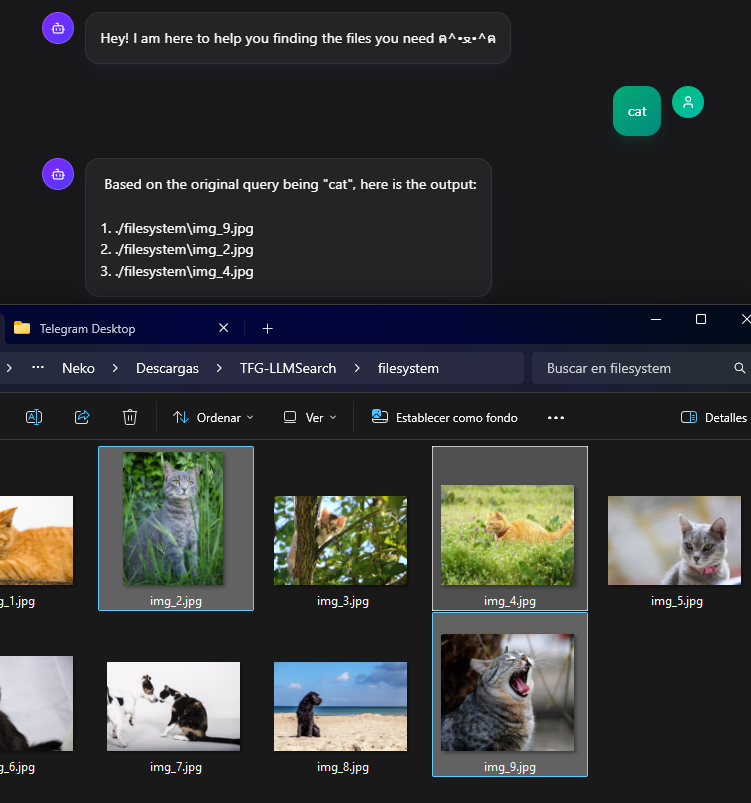
\includegraphics[width=0.9\textwidth]{archivos/cats_dataset_result.png}
\caption[Resultados de búsqueda para "cat"]{Resultados de la búsqueda para la consulta "cat", mostrando tres imágenes de gatos.}
\label{fig:cats_search_results}
\end{figure}

En la búsqueda de "dog", los resultados iniciales de ChromaDB fueron pertinentes. Sin embargo, el modelo Mistral, encargado de refinar y presentar estos resultados, introdujo un error: aunque el número total de perros identificados fue el esperado, el primer resultado mostrado fue incorrecto (un gato en lugar de un perro), como se ilustra en la Figura \ref{fig:dogs_search_results_error}. Los logs de Prefect (Figura \ref{fig:dogs_prefect_results_correct}) confirmaron que la selección de ChromaDB sí era más acertada antes del paso por Mistral mostrando en este orden las imágenes 7(perro), 8(perro) y 4(gato).

\begin{figure}[H]
\centering
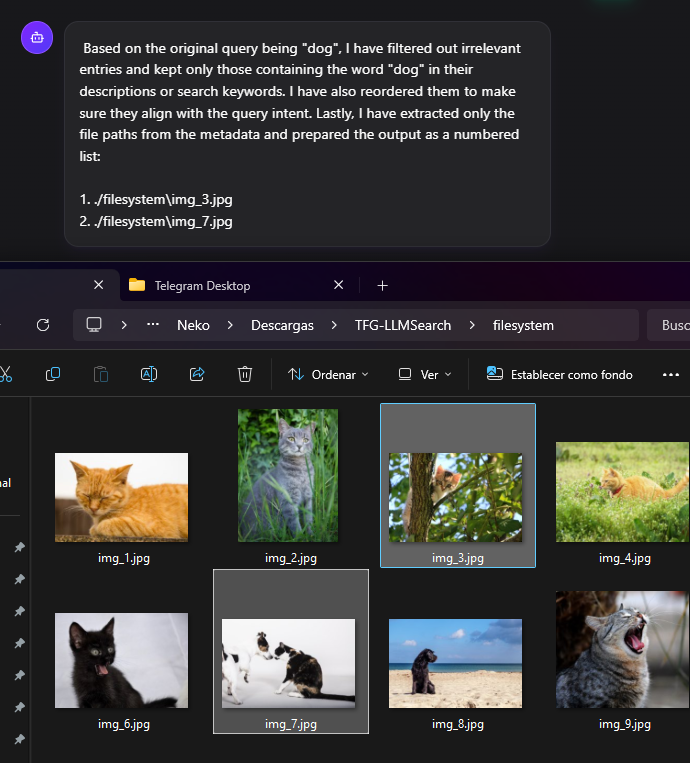
\includegraphics[width=0.9\textwidth]{archivos/dogs_result.png}
\caption[Resultados de búsqueda para "dog" con error]{Resultados de la búsqueda para "dog", donde el primer resultado es incorrecto debido al post-procesamiento de Mistral.}
\label{fig:dogs_search_results_error}
\end{figure}

\begin{figure}[H]
\centering
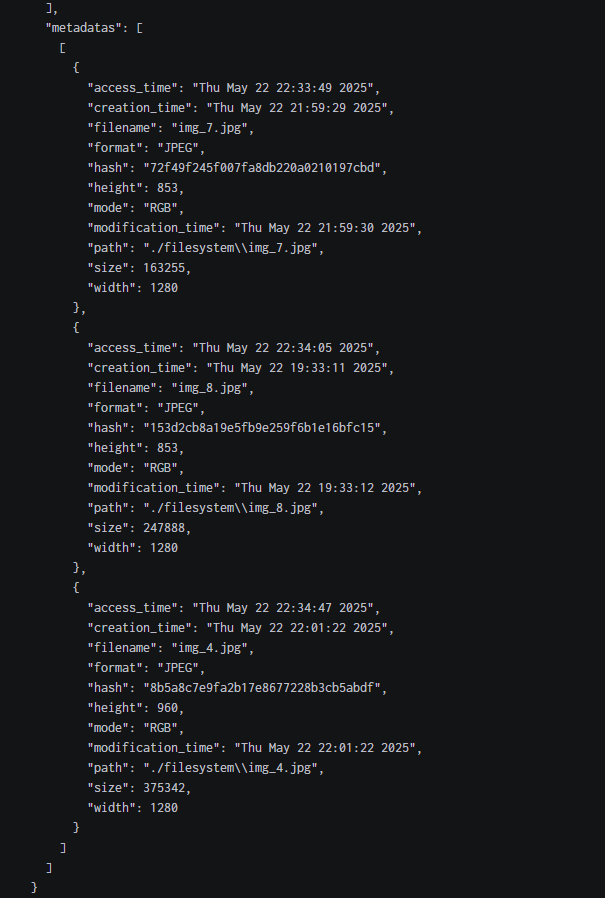
\includegraphics[width=0.9\textwidth]{archivos/dogs_prefect_result.png}
\caption[Resultados de ChromaDB para "dog" en Prefect]{Vista de Prefect mostrando los resultados (más precisos) de ChromaDB para la consulta "dog" antes del filtro de Mistral.}
\label{fig:dogs_prefect_results_correct}
\end{figure}

Finalmente, se realizó una prueba con la consulta "orange cat". En este caso, ChromaDB identificó correctamente los gatos naranjas disponibles. No obstante, el modelo Mistral nuevamente falló en el filtrado y presentación final, mostrando solo uno de los gatos naranjas relevantes (Figura \ref{fig:orange_cat_search_result_error}), a pesar de que los resultados intermedios de ChromaDB (visibles en Prefect, Figura \ref{fig:orange_cat_prefect_result_correct}) eran más completos mostrando en este orden los gatos 4(naranja), 1(naranja) y 5(gris).

\begin{figure}[H]
\centering
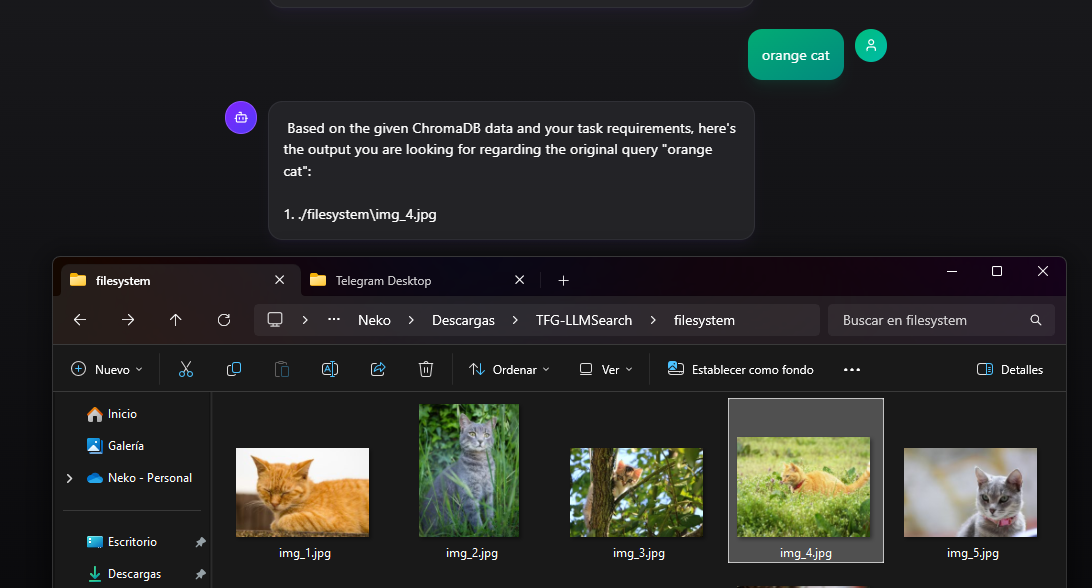
\includegraphics[width=0.9\textwidth]{archivos/orange_cat_result.png}
\caption[Resultados de búsqueda para "orange cat" con error]{Resultado de la búsqueda para "orange cat", mostrando un solo gato naranja debido al filtrado de Mistral.}
\label{fig:orange_cat_search_result_error}
\end{figure}

\begin{figure}[H]
\centering
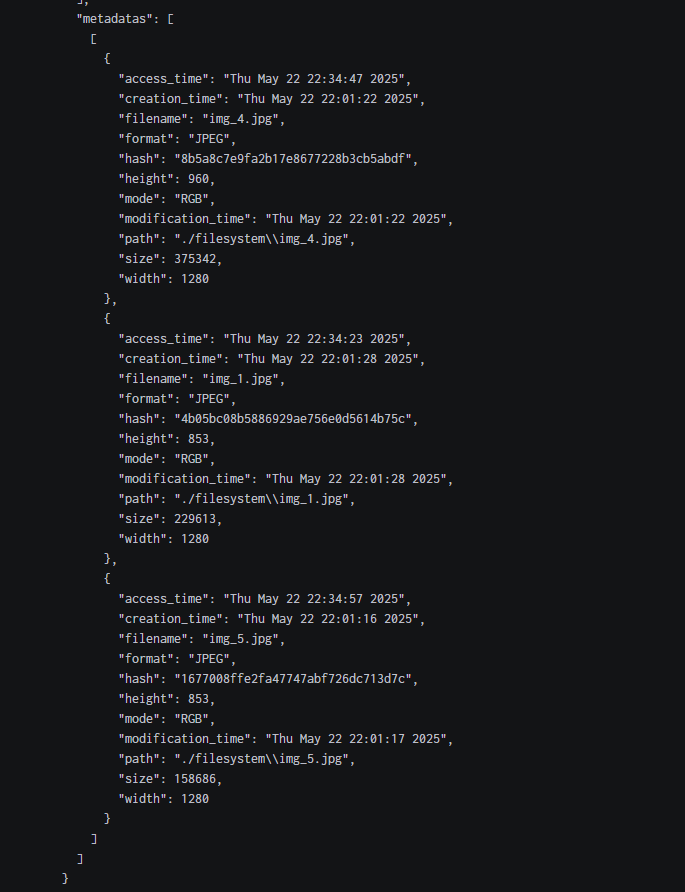
\includegraphics[width=0.9\textwidth]{archivos/orange_cat_prefect_result.png}
\caption[Resultados de ChromaDB para "orange cat" en Prefect]{Vista de Prefect que muestra los resultados más precisos de ChromaDB para "orange cat" antes del post-procesamiento de Mistral.}
\label{fig:orange_cat_prefect_result_correct}
\end{figure}

Estas pruebas con el dataset mixto revelan que, si bien la base de datos vectorial ChromaDB realiza una recuperación semántica inicial efectiva, el rendimiento del modelo de lenguaje (Mistral) utilizado para el refinamiento o la generación de la respuesta final puede ser un punto crítico, introduciendo errores o perdiendo información relevante en algunos casos, especialmente con metadatos extensos o en tareas de filtrado fino.

\subsubsection{Gemma3 como modelo final de lenguaje}
\label{sec:gemma3_test}

Para comparar el rendimiento y la precisión de Mistral con otro modelo de lenguaje, se repitió la búsqueda de "dog" utilizando el modelo Gemma3 dando los siguientes resultados (Figura \ref{fig:gemma3_dogs_search_results}):
\begin{figure}[H]
\centering
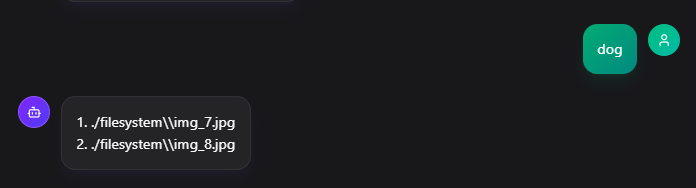
\includegraphics[width=0.9\textwidth]{archivos/gemma3_dogs_result.png}
\caption[Resultados de búsqueda para "dog" con Gemma3]{Resultados de la búsqueda para "dog" utilizando el modelo Gemma3, mostrando los dos perros correctamente.}
\label{fig:gemma3_dogs_search_results}
\end{figure}

Los resultados obtenidos con Gemma3 fueron correctos, mostrando los dos perros existentes. Esto sugiere que el modelo Gemma3 podría ser una mejor opción para la tarea de búsqueda semántica en comparación con Mistral, sin embargo, el modelo Mistral ha tardado 3 segundos en procesar la consulta mientras que Gemma3 ha tardado 1 minutos y medio en procesar la misma consulta incluso dejando el equipo congelado durante algunos momentos. Esto sugiere que, aunque Gemma3 puede ofrecer resultados más precisos, su tiempo de respuesta es significativamente mayor, lo que podría ser un inconveniente en aplicaciones donde la velocidad es crítica.
\begin{figure}[H]
\centering
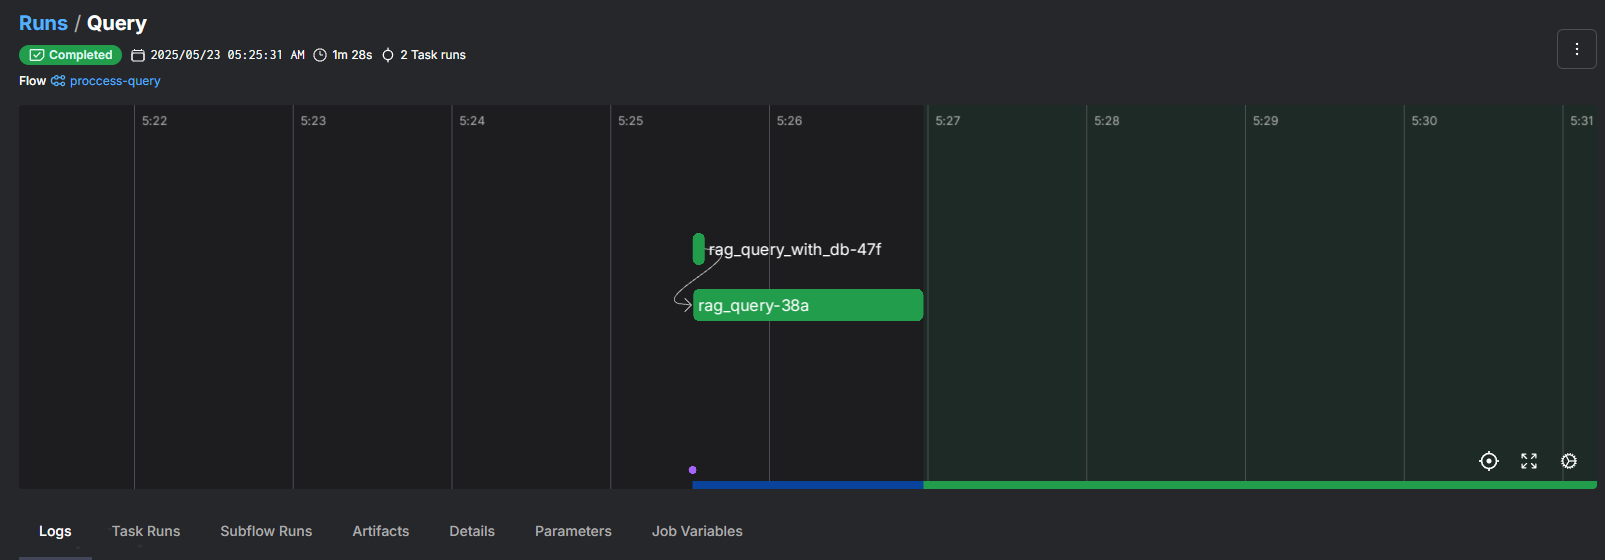
\includegraphics[width=0.9\textwidth]{archivos/gemma3_time.png}
\caption[Tiempo de respuesta de Gemma3]{Tiempo de respuesta del modelo Gemma3 al procesar la consulta "dog".}
\label{fig:gemma3_time}
\end{figure}

\subsection{Ejecución sin GPU}
\label{sec:execution_without_gpu}
Uno de los objetivos opcionales del proyecto era la posibilidad de ejecutar el sistema en un entorno sin GPU, lo que sería útil para usuarios en dispositivos móviles.
Gemma3, al ser un modelo grande es imposible de ejecutar sin GPU, pero Mistral puede ejecutarse en CPU desactivando la opción de GPU en LMStudio.

\begin{figure}[H]
\centering
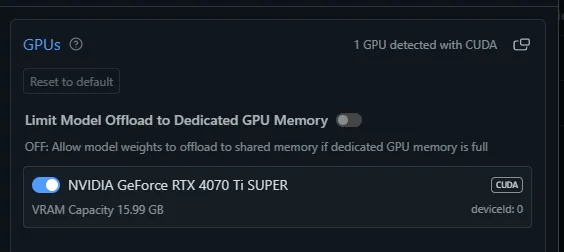
\includegraphics[width=0.9\textwidth]{archivos/no_gpu.png}
\caption[Ejecución de Mistral sin GPU]{Ejecución del modelo Mistral en CPU, mostrando el uso de recursos del sistema.}
\label{fig:no_gpu}
\end{figure}

Se repitió la búsqueda de "dog" utilizando el modelo Mistral en CPU, y los resultados fueron los mismos que los obtenidos con GPU con la diferencia de que el tiempo de respuesta ha sido de 42 segundos frente a los 3 segundos que tardó en GPU. Esto demuestra que el sistema es capaz de funcionar sin GPU, pero el tiempo de respuesta es significativamente mayor, lo que podría ser un inconveniente en aplicaciones donde la velocidad es crítica.
\begin{figure}[H]
\centering
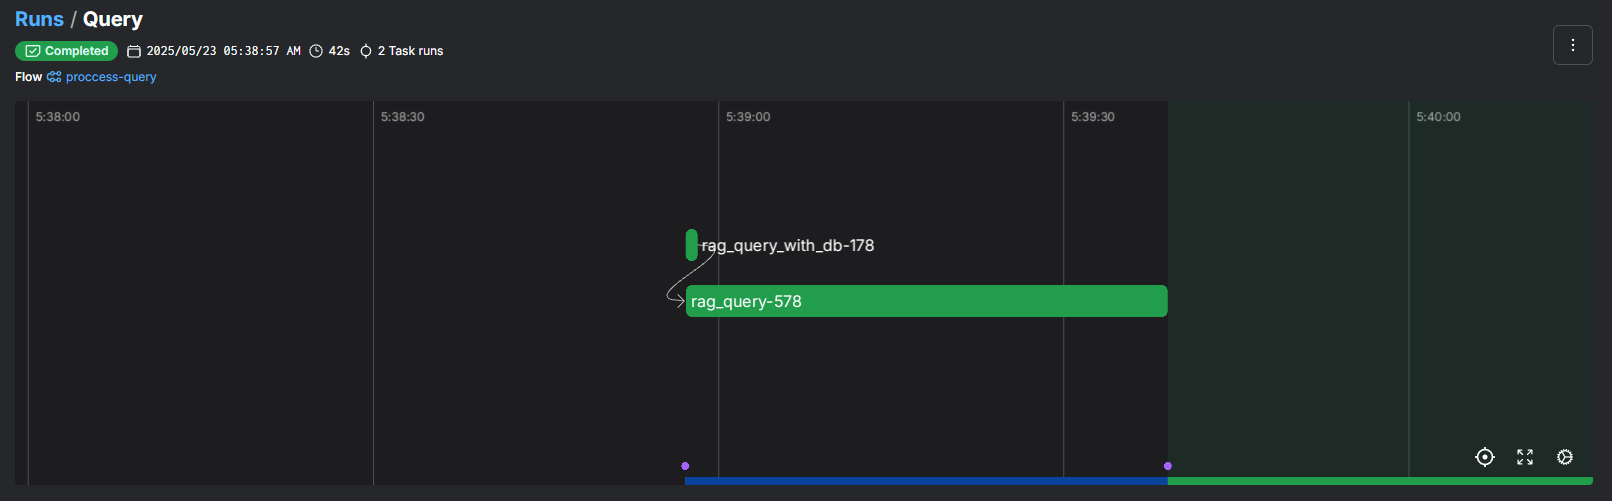
\includegraphics[width=0.9\textwidth]{archivos/no_gpu_time.png}
\caption[Tiempo de respuesta de Mistral sin GPU]{Tiempo de respuesta del modelo Mistral al procesar la consulta "dog" en CPU.}
\label{fig:no_gpu_time}
\end{figure}
